% =============================================================
%  SECTION: Module 5 — Initialization, Equilibration & Assembly
%  ASSIGNED TO: [Person Name]
%
%  GUIDING QUESTIONS TO ANSWER:
%   WHAT  — What is the Maxwell-Boltzmann distribution?
%           What is velocity rescaling? What is equilibration?
%   WHY   — Why can't we just give all atoms the same speed?
%           Why zero the net momentum before running?
%           Why run an equilibration phase before collecting data?
%   HOW   — How is Gaussian sampling used to initialise velocities?
%           How does the rescaling thermostat work (lambda factor)?
%           What are the equilibration and production phases?
%  EXTRAS — Energy compensation: K* and U* oscillate anti-phase.
%           Plot of K*, U*, E* all on one graph.
%           What happens to E* during equilibration vs production?
% =============================================================
% =============================================================
%  SECTION: Module 5 — Initialization, Equilibration & Assembly
% =============================================================

\newpage
\section{Module 5: Initialization, Equilibration, and System Assembly}

\subsection{What Are We Doing?}

Having built the tools to compute forces (Module 1), enforce periodic geometry (Module 2), propagate motion (Module 3), and do so efficiently (Module 4), we are now ready to assemble them into a working simulation. But before the engine can run, we must answer two questions that every real physicist faces when setting up an experiment: \emph{how do we prepare the system in a physically valid state?} and \emph{how long do we wait before we trust any measurement?}

This module solves both problems. It assigns every atom a velocity drawn from the correct statistical distribution for the target temperature, eliminates any spurious centre-of-mass drift, and then runs an equilibration phase — a controlled warm-up period — before the simulation settles into the stable state from which we collect data.

\subsection{Why Are We Doing It?}

\subsubsection{Why Maxwell-Boltzmann Velocities?}

Imagine you are running at a temperature $T^*$ and you need to assign each atom a starting speed. The naive approach — give every atom exactly the same speed — creates an artificial, crystalline structure in velocity space that does not resemble any real material. In reality, atoms in thermal equilibrium do not move uniformly. Some are slow, some are fast, and their speeds span a continuous range set by the \textbf{Maxwell-Boltzmann distribution} — a direct consequence of classical statistical mechanics.

This distribution tells us that each individual velocity component ($v_x$, $v_y$, $v_z$) of any given atom is a Gaussian random variable with zero mean and a spread determined entirely by temperature. In reduced units, the standard deviation is simply $\sigma = \sqrt{T^*}$: hotter systems have faster, more spread-out velocity distributions. By sampling each component from this Gaussian, we start the simulation as close as possible to a real thermal equilibrium — no artificial symmetry, no unphysical ordering.

\subsubsection{Why Zero the Net Momentum?}

When $N$ velocities are drawn at random from a Gaussian, the sum will not be exactly zero — statistical fluctuations guarantee a small, nonzero net momentum $\mathbf{P}^* = \sum_i \mathbf{v}_i$. This is harmless in nature (where there is no preferred reference frame), but in a simulation it is catastrophic. A nonzero total momentum means the entire collection of atoms is slowly drifting in one direction, as if the whole simulation box were a single projectile. Over time, atoms leave one side of the periodic cell faster than they re-enter from the other, breaking the statistical homogeneity that makes PBC valid.

The fix is one line: subtract the mean velocity from every atom before the simulation begins. This zeroes $\mathbf{P}^*$ exactly and anchors the centre of mass permanently to rest.

\subsubsection{Why an Equilibration Phase?}

We begin on a perfect FCC lattice — every atom sitting precisely at its ideal lattice site, none of them where they would actually be in a thermodynamically equilibrated solid or liquid. This is a highly artificial initial condition: the atoms have not yet had time to settle into their natural configurations, and the kinetic and potential energies are far from their equilibrium balance.

If we were to start collecting data immediately, every measurement would be contaminated by this transient. The $g(r)$ would reflect the perfect FCC geometry rather than true thermal structure; the energy would still be drifting toward its equilibrium value. The equilibration phase gives the system time to relax: we run the integrator while periodically forcing the temperature back to its target value, letting the atoms reorganise while guiding the system toward equilibrium. Once the energies have settled into steady oscillations and the temperature is stable, we switch off the thermostat and let the system run freely — this is the production phase, and only now do we trust the data.

\subsection{How Is It Implemented?}

\subsubsection{Velocity Initialization}

Each velocity component $v_{i\alpha}$ is sampled independently from a Gaussian:
\begin{equation}
    \rho(v_{i\alpha}) = \frac{1}{\sigma\sqrt{2\pi}}\exp\!\left(-\frac{v_{i\alpha}^2}{2\sigma^2}\right),
    \quad \sigma = \sqrt{\Tstar}
    \label{eq:mb}
\end{equation}
After sampling, the mean velocity is subtracted component-wise so that $\sum_i \mathbf{v}_i = \mathbf{0}$ exactly. In our test run, the residual momentum after this step was $|\mathbf{P}^*| = 1.77 \times 10^{-14}$ — numerical noise at the level of floating-point precision.

\subsubsection{Velocity Rescaling Thermostat}

At any instant during the simulation, the instantaneous reduced temperature is directly related to the total kinetic energy:
\begin{equation}
    \Tstar_{\text{inst}} = \frac{1}{3N}\sum_i |\mathbf{v}_i^*|^2
    \label{eq:T_inst}
\end{equation}
To steer the system toward a target $\Tstar_{\text{target}}$, all velocities are multiplied by a single scaling factor $\lambda$:
\begin{equation}
    \lambda = \sqrt{\frac{\Tstar_{\text{target}}}{\Tstar_{\text{inst}}}}
    \qquad\Rightarrow\qquad
    \mathbf{v}_i^{\text{new}} = \lambda\,\mathbf{v}_i
    \label{eq:rescale}
\end{equation}
This works because kinetic energy scales as $v^2$: multiplying every speed by $\lambda$ multiplies $K^*$ by $\lambda^2 = T_{\text{target}}/T_{\text{inst}}$, exactly reaching the target. Rescaling is applied every 10 steps during the equilibration phase; it is switched off entirely during production so the system evolves freely in the NVE ensemble.

\subsubsection{The Master MD Loop}

The complete simulation proceeds in three stages:

\begin{enumerate}
    \item \textbf{Initialise:} Generate the FCC lattice (Module 2), assign Maxwell-Boltzmann velocities, zero net momentum, build the initial Verlet neighbour list (Module 4), and compute the initial forces.
    \item \textbf{Equilibration} (steps 0 to $N_{\text{equil}}$): Advance with the Velocity Verlet integrator (Module 3 via Module 4); apply velocity rescaling every 10 steps to hold $T^* \approx T_{\text{target}}$. No data is recorded.
    \item \textbf{Production} (steps $N_{\text{equil}}$ to $N_{\text{total}}$): Thermostat is switched off. The system evolves freely; all energies, temperatures, and structural observables are accumulated.
\end{enumerate}

In this module test we ran $N_{\text{total}} = 5000$ steps with a 50/50 equilibration-to-production split: 2500 equilibration steps followed by 2500 production steps.

\subsection{Energy Compensation: A Key Diagnostic}

As the system relaxes from the perfect FCC lattice during equilibration, the potential and kinetic energies exchange rapidly — $K^*$ rises when atoms fly apart as the lattice melts thermally, and $U^*$ falls correspondingly. These fluctuations are not noise; they are the fundamental exchange between kinetic and potential energy that every classical system undergoes. The critical test is whether they cancel: in a physically correct simulation, every joule that leaves $U^*$ must appear in $K^*$ and vice versa, keeping $E^* = K^* + U^*$ flat. During equilibration, the periodic velocity rescaling will cause visible step-like jumps in $E^*$ as kinetic energy is injected or removed. These jumps vanish completely once the thermostat is switched off and production begins.

\begin{figure}[H]
    \centering
    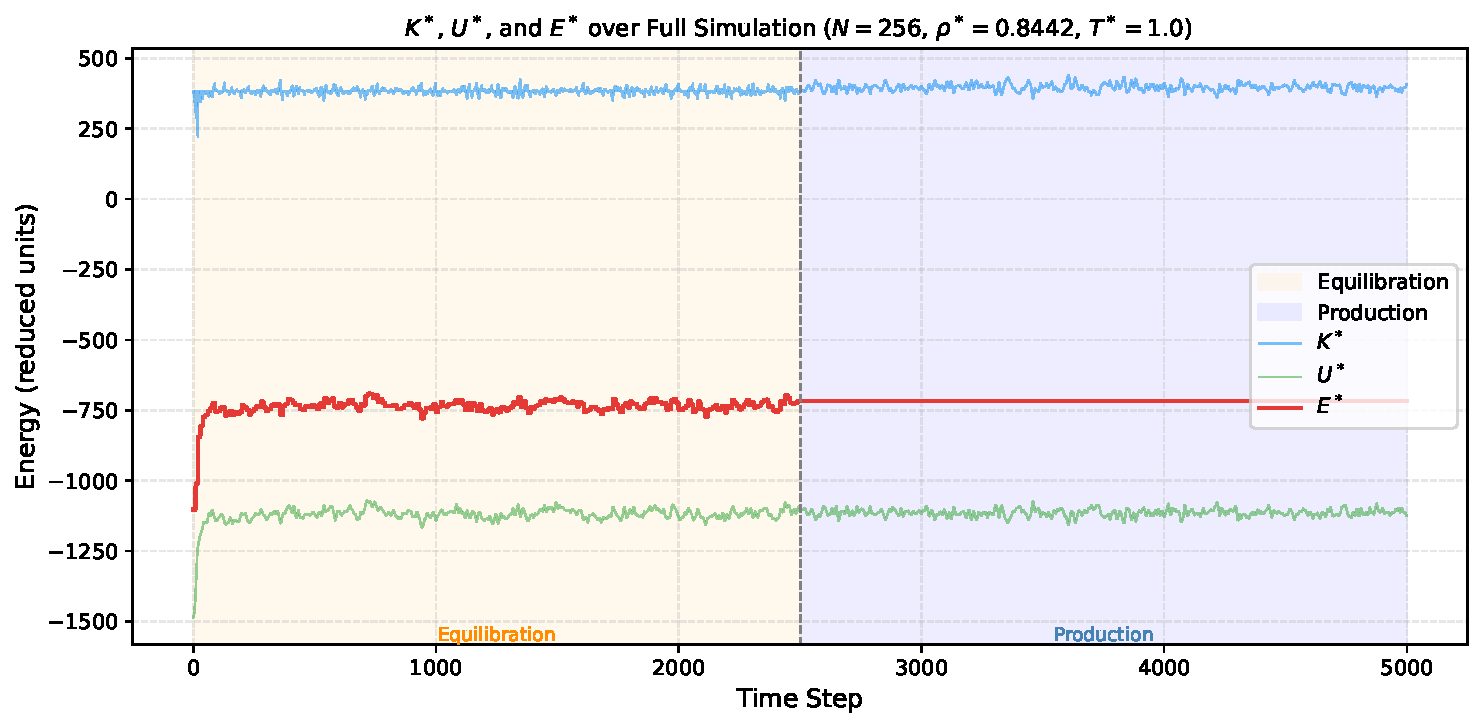
\includegraphics[width=\linewidth]{figures/m5_energy_three_panel.pdf}
    \caption{Kinetic energy $K^*$, potential energy $U^*$, and total energy $E^*$ over all 5000 timesteps for $N=256$, $\rho^* = 0.8442$, $T^* = 1.0$, $\delta t^* = 0.005$. The orange-shaded region is the equilibration phase (steps 0--2500), where velocity rescaling periodically adjusts $K^*$; the blue-shaded region is the production phase (steps 2500--5000), where all quantities evolve freely. The flatness of $E^*$ (red) in the production phase is the primary confirmation of physical correctness.}
    \label{fig:m5_energy}
\end{figure}

\begin{figure}[H]
    \centering
    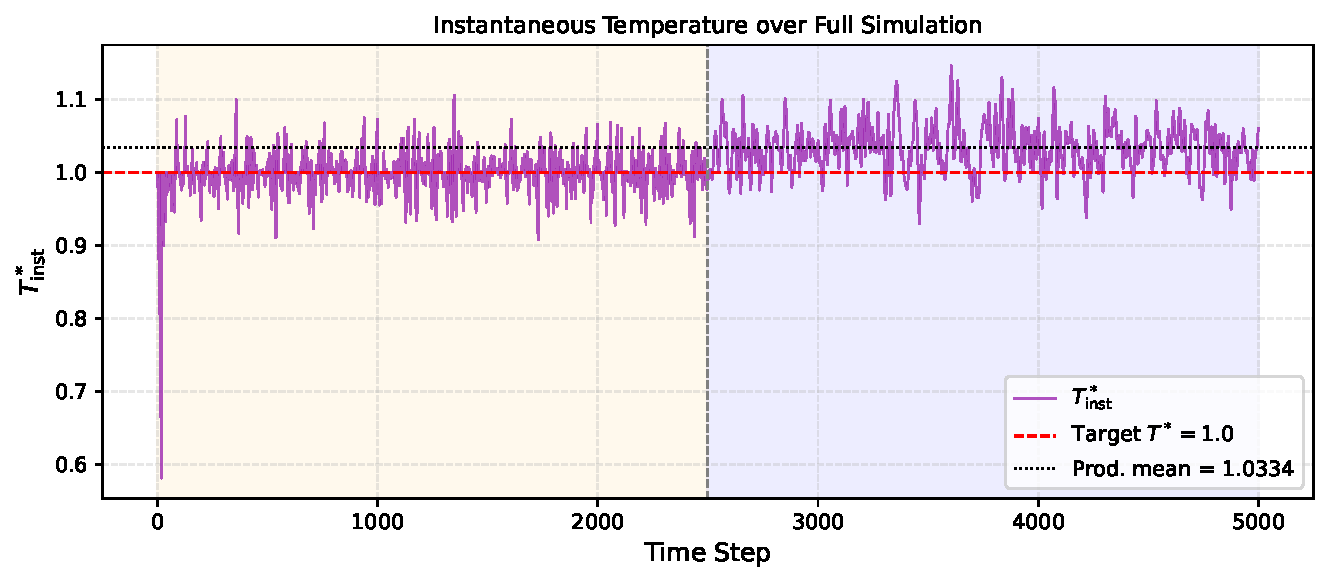
\includegraphics[width=0.9\linewidth]{figures/m5_temperature.pdf}
    \caption{Instantaneous reduced temperature $T^*_\text{inst}$ over all 5000 timesteps. During equilibration the thermostat clamps the temperature tightly to the target $T^* = 1.0$ (red dashed); in production it fluctuates naturally around $\langle T^* \rangle = 1.033$ (black dotted), a small deviation from 1.0 that reflects the finite-size statistical nature of the NVE ensemble after thermostat removal.}
    \label{fig:m5_temp}
\end{figure}

\subsection{Test Results}

\begin{table}[H]
    \centering
    \caption{Module 5 verification for $N = 256$, $\rhostar = 0.8442$, $\Tstar = 1.0$, $\delta t^* = 0.005$, 5000 total steps (2500 equilibration + 2500 production).}
    \label{tab:m5_test}
    \begin{tabular}{lcc}
        \toprule
        \textbf{Quantity} & \textbf{Expected} & \textbf{Measured} \\
        \midrule
        $\langle \Tstar \rangle$ (production)              & $\approx 1.0$         & $1.033$ \\
        Initial $|\mathbf{P}^*|$ after zeroing             & $\approx 0$           & $1.77 \times 10^{-14}$ \\
        Max $|P_x^*|$ during run                           & $\approx 0$           & $1.49 \times 10^{-13}$ \\
        Max $|P_y^*|$ during run                           & $\approx 0$           & $1.16 \times 10^{-13}$ \\
        Max $|P_z^*|$ during run                           & $\approx 0$           & $1.57 \times 10^{-13}$ \\
        $\langle \Estar \rangle$ (production)              & ---                   & $-717.16$ \\
        RMS fluctuation $\Delta \Estar$                    & ---                   & $5.34 \times 10^{-2}$ \\
        Relative fluctuation $\Delta \Estar/|\langle \Estar \rangle|$ & $\lesssim 10^{-4}$ & $7.45 \times 10^{-5}$ \\
        Criterion met?                                      & ---                   & \textbf{Yes} \\
        \bottomrule
    \end{tabular}
\end{table}

All three diagnostic criteria are satisfied. The total momentum components remain at machine-precision levels ($\sim 10^{-13}$) throughout the entire run — they never grow, confirming that the momentum-zeroing step and the Velocity Verlet integrator both preserve $\mathbf{P}^* = \mathbf{0}$ exactly. The relative energy fluctuation of $7.45 \times 10^{-5}$ falls below the $10^{-4}$ threshold, confirming that $\delta t^* = 0.005$ is a stable choice. The production-phase temperature of $\langle T^* \rangle = 1.033$ sits slightly above the target of $1.0$; this is expected and physically correct — once the rescaling thermostat is removed, the NVE ensemble conserves energy rather than temperature, and finite-size fluctuations allow the mean temperature to settle at a value slightly different from the target. The system is in equilibrium, and production data is trustworthy.